\documentclass[11pt,letterpaper]{article}
\usepackage[lmargin=1in,rmargin=1in,tmargin=1in,bmargin=1in]{geometry}
\usepackage{../style/homework}
\usepackage{../style/commands}
\setbool{quotetype}{true} % True: Side; False: Under
\setbool{hideans}{false} % Student: True; Instructor: False

% -------------------
% Content
% -------------------
\begin{document}

\homework{11: Due 11/06}{Learning is not attained by chance; it must be sought for with ardor and attended to with diligence.}{Abigail Adams}

% Problem 1
\problem{10} Find the equation of the line plotted below.
	\[
	\fbox{
	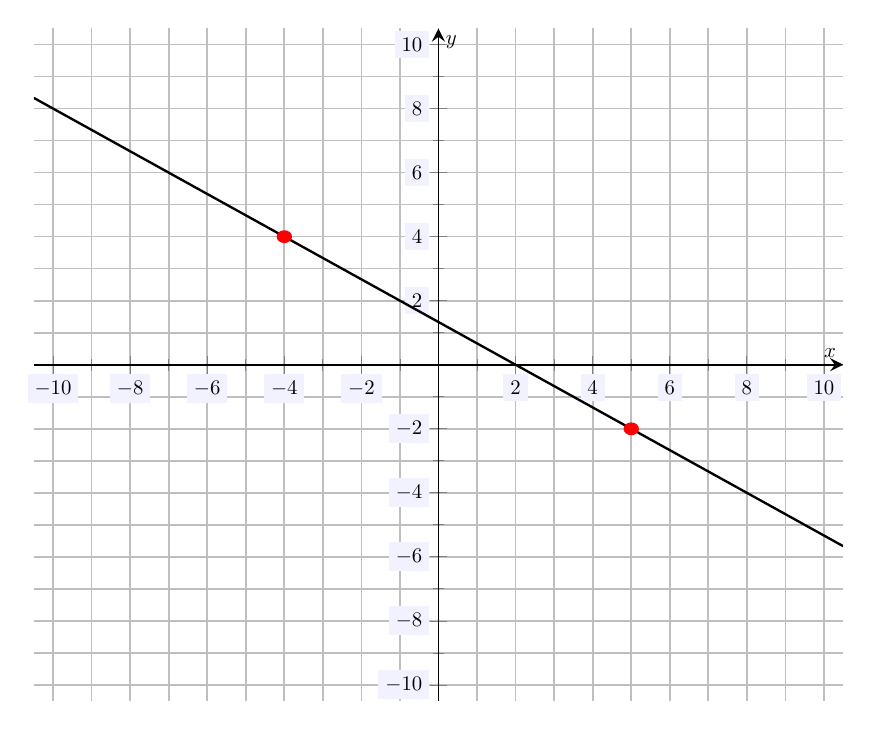
\begin{tikzpicture}[scale=1.5,every node/.style={scale=0.5}]
	\begin{axis}[
	grid=both,
	axis lines=middle,
	ticklabel style={fill=blue!5!white},
	xmin= -10.5, xmax=10.5,
	ymin= -10.5, ymax=10.5,
	xtick={-10,-8,-6,-4,-2,0,2,4,6,8,10},
	ytick={-10,-8,-6,-4,-2,0,2,4,6,8,10},
	minor tick = {-10,-9,...,10},
	xlabel=\(x\),ylabel=\(y\),
	]
	\addplot[line width= 0.02cm,samples=2,domain= -10.5:10.5] ({x},{4/3 - 2/3*x});
	\draw[fill=red,draw=none] (-4,4) circle (0.2);
	\draw[fill=red,draw=none] (5,-2) circle (0.2);
	\end{axis}
	\end{tikzpicture}
	}
	\] \pspace

\sol Because this line is a linear function, we know that the line has the form $y= mx + b$. From the plot above, we can see that the points $(-4, 4)$ and $(5, -2)$ are on the line. We can then determine the slope of the line:
	\[
	m= \dfrac{\Delta y}{\Delta x}= \dfrac{4 - (-2)}{-4 - 5}= \dfrac{4 + 2}{-4 + -5}= \dfrac{6}{-9}= -\dfrac{2}{3}
	\]
But then $y= -\frac{2}{3}\,x + b$. Because the line contains the point $(-4, 4)$, the point satisfies the equation for the line. But then\dots
	\[
	\begin{gathered}
	y= -\dfrac{2}{3}\,x + b \\
	4= -\dfrac{2}{3} \cdot -4 + b \\
	4= \dfrac{8}{3} + b \\
	b= \dfrac{4}{3}
	\end{gathered}
	\]
Alternatively, we can use the point-slope form of a linear function:
	\[
	y= y_0 + m(x - x_0)= 4 + \dfrac{-2}{3} \big(x - (-4) \big)= 4 - \dfrac{2}{3} (x + 4)= 4 - \dfrac{2}{3}\,x - \dfrac{8}{3}= -\dfrac{2}{3}\,x + \dfrac{4}{3}
	\]	
Therefore, the equation of the line is $y= -\frac{2}{3}\,x + \frac{4}{3}$.



\newpage



% Problem 2
\problem{10} Find the equation of the line containing the point $(-5, 6)$ with slope $-\frac{1}{3}$. \pspace

\sol Clearly, the line is not vertical. Therefore, the line must have the form $y= mx + b$. Because the line has slope $-\frac{1}{3}$, we have $m= -\frac{1}{3}$. Then we know $y= -\frac{1}{3}\,x + b$. Because the line contains the point $(-5, 6)$, it satisfies the equation of the line. But then\dots
	\[
	\begin{gathered}
	y= -\dfrac{1}{3}\,x + b \\
	6= -\dfrac{1}{3} \cdot -5 + b \\
	6= \dfrac{5}{3} + b \\
	b= \dfrac{13}{3}
	\end{gathered}
	\]
Alternatively, we can use the point-slope form of the line:
	\[
	y= y_0 + m(x - x_0)= 6 + \dfrac{-1}{3} \big(x - (-5) \big)= 6 - \dfrac{1}{3} (x + 5)= 6 - \dfrac{1}{3}\,x - \dfrac{5}{3}= -\dfrac{1}{3}\,x + \dfrac{13}{3}
	\]
Therefore, the line is $y= -\frac{1}{3}\,x + \frac{13}{3}$.



\newpage



% Problem 3
\problem{10} Find the equation of the line with $x$-intercept 5 and $y$-intercept $-6$. \pspace

\sol Clearly, the line is not vertical. Therefore, the line has the form $y= mx + b$. Because the line contains the $x$ and $y$-intercept, the line contain the point $(5, 0)$ and $(0, -6)$, respectively. But then we can compute the slope of the line:
	\[
	m= \dfrac{\Delta y}{\Delta x}= \dfrac{0 - (-6)}{5 - 0}= \dfrac{0 + 6}{5 - 0}= \dfrac{6}{5}
	\]
But then $y= \frac{6}{5}\,x + b$. Because the line contains the point $(0, -6)$, the point satisfies the equation for the line. But then\dots
	\[
	\begin{gathered}
	y= \dfrac{6}{5}\,x + b \\
	-6= \dfrac{6}{5} \cdot 0 + b \\
	b= -6
	\end{gathered}
	\]
Of course, we could note that $b$ is the $y$-intercept so that $b= -6$. Alternatively, we can use the point-slope form of a linear function:
	\[
	y= y_0 + m(x - x_0)= -6 + \dfrac{6}{5} (x - 0)= \dfrac{6}{5}\,x - 6
	\]	
Therefore, the equation of the line is $y= \frac{6}{5}\,x - 6$. 



\newpage



% Problem 4
\problem{10} Find the equation of the line parallel to the line $\ell(x)= \frac{4 - x}{6}$ whose $x$-intercept is $(9, 0)$. \pspace

\sol Because the line $\ell(x)$ is not vertical, it must be that the line in question is not vertical. Therefore, the line has the form $y= mx + b$. Because the line is parallel to the line $\ell(x)$, it must have the same slope as $\ell(x)$. The line $\ell(x)= \frac{4 - x}{6}= \frac{4}{6} - \frac{1}{6}\,x$ has slope $-\frac{1}{6}$. Therefore, we must have $m= -\frac{1}{6}$. Then we know $y= -\frac{1}{6}\,x + b$. Because the line contains the point $(9, 0)$, it must satisfy the equation of the line. But then\dots
	\[
	\begin{gathered}
	y= -\dfrac{1}{6}\,x + b \\
	0= -\dfrac{1}{6} \cdot 9 + b \\
	0= -\dfrac{3}{2} + b \\
	b= \dfrac{3}{2}
	\end{gathered}
	\]
Alternatively, we can use the point-slope form of the line:
	\[
	y= y_0 + m(x - x_0)= 0 + \dfrac{-1}{6} (x - 9)= -\dfrac{1}{6}\,x + \dfrac{3}{2}
	\]
Therefore, the line is $y= -\frac{1}{6}\,x + \frac{3}{2}= \frac{9 - x}{6}$.


\end{document}